\documentclass[journal=jacsat,manuscript=article]{achemso}
\usepackage[version=3]{mhchem}
\usepackage{amsmath}
\usepackage{ctex}
\usepackage{longtable}
\usepackage{booktabs}
\newcommand*\mycommand[1]{\texttt{\emph{#1}}}
\providecommand{\tightlist}{%
  \setlength{\itemsep}{0pt}\setlength{\parskip}{0pt}}
\author{蓝海}
\altaffiliation{我们认真科学分析金融的规律}
\email{lh_loki@163.com}
\phone{13127900572}
\author{彭莉}


\keywords{价值投资, PB-ROE}

\title[曹名长]{曹名长简评\footnote{详尽的数据分析与记录请联系作者索取《基金管理人分析技术文档》}}
\makeatletter
\ifxetex
  \usepackage[setpagesize=false, % page size defined by xetex
              unicode=false, % unicode breaks when used with xetex
              xetex]{hyperref}
\else
  \usepackage[unicode=true]{hyperref}
\fi
\hypersetup{breaklinks=true,
            bookmarks=true,
            pdfauthor={},
            pdftitle={},
            colorlinks=true,
            urlcolor=blue,
            linkcolor=magenta,
            pdfborder={0 0 0}}
\urlstyle{same}  % don't use monospace font for urls
% pandoc header

\begin{document}
\begin{abstract}
曹名长是市场上价值投资的长跑健将。在长达15年的证券行业从业经历中,以基金经理人的身份长期管理多只偏股混合型基金,取得了不俗的投资收益。

基于公开信息分析,我们认为曹名长是典型的长线、分散型价值投资者,其具备较强的选股能力和一定的行业配置能力,长期保持低换手率和偏稳健的主动策略,持续的投资于低估值、成长性确定的大中盘价值股。
随着市场风格的改变,曹名长不断的调整选择投资对象的一些风格属性,如PB、PE等,但是不变的是其在各种市场压力下坚持长线、坚持价值优先的投资理念。他是``进化型''的价值投资者。
\end{abstract}
\begin{figure}[htbp]
\centering
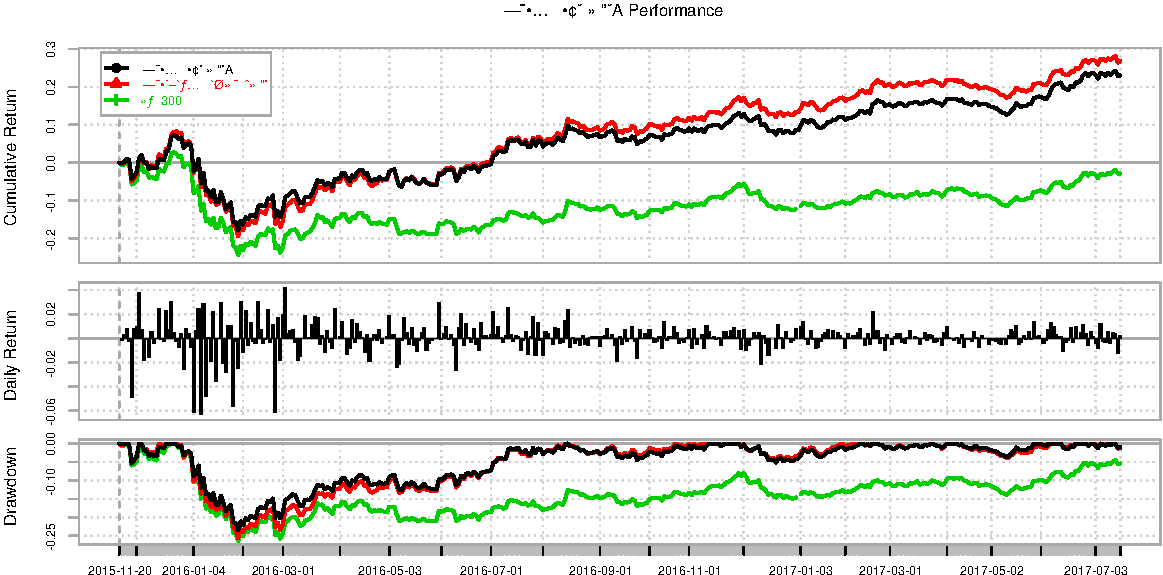
\includegraphics[width=15cm]{cmc-review_files/figure-latex/unnamed-chunk-1-1.pdf}
\caption{基金累计回报率与回撤}
\end{figure}

\begin{longtable}[]{@{}llclclc@{}}
\toprule
名称 & 近半年 & 夏普率 & 近一年 & 夏普率 & 近两年 &
夏普率\tabularnewline
\midrule
\endhead
中欧价值发现混合A & 10.8\% & 2.1 & 24\% & 0.57 & 23.0\% &
0.49\tabularnewline
中欧潜力价值灵活配置混合 & 9.7\% & 1.9 & 26\% & 0.65 & 26.8\% &
0.57\tabularnewline
沪深300 & 8.9\% & 1.6 & 16\% & -0.22 & -2.9\% & -0.29\tabularnewline
\bottomrule
\end{longtable}

\begin{figure}[htbp]
\centering
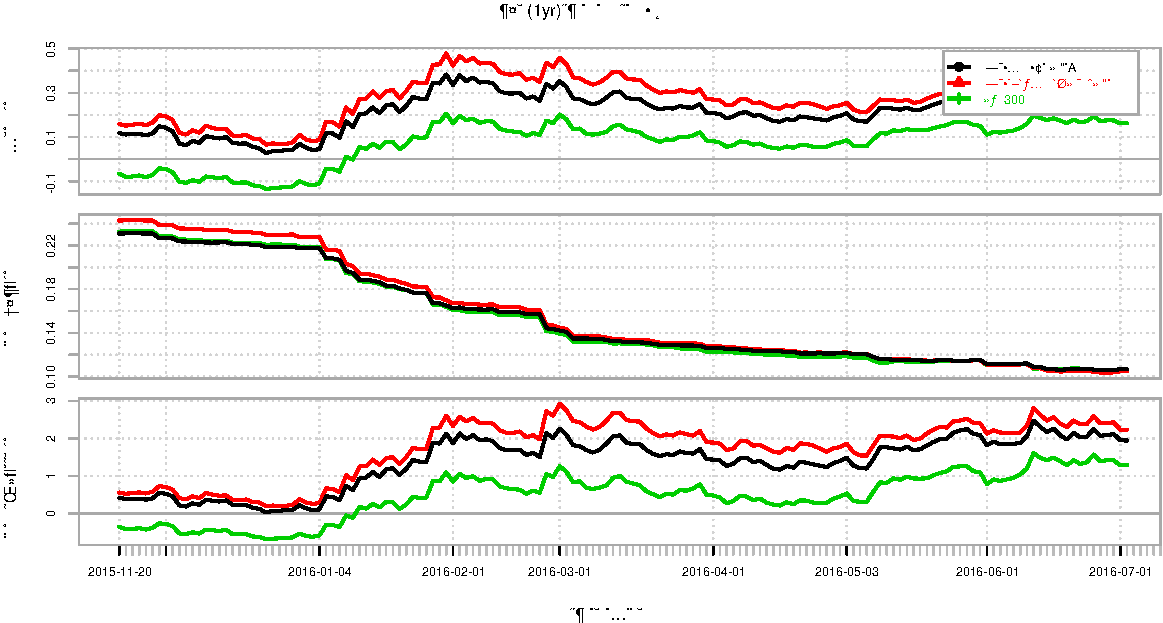
\includegraphics[width=15cm]{cmc-review_files/figure-latex/unnamed-chunk-2-1.pdf}
\caption{投资者收益风险比较}
\end{figure}

\section{简介}

上海财经大学计量经济学硕士。历任君安证券公司研究所研究员,闽发证券上海研发中心研究员,红塔证券资产管理总部投资经理,百瑞信托有限责任公司信托经理,新华基金管理公司总经理助理、基金经理。2015年6月加入中欧基金管理有限公司,现任事业部负责人、基金经理。

\section{风格评述}

曹名长的风格集中表现为:

\begin{itemize}
\item 交易风格:非常低的换手率,长期持股;
\item 持仓风格:大盘、价值是其持仓的主线,但是价值不是绝对价值,而更多考虑相对价值,会给予确定性的成长相应的溢价;
\item 主动性风格:主动指数17%,曹名长的管理风格可以定义为稳健的主动管理型。
\end{itemize}

\section{\texorpdfstring{能力评价\footnote{运气能够带来超常表现,持续的好运则可以归结为能力!}}{能力评价}}

我们讲持续的超额表现归因为

\begin{equation}
\mbox{大类资产配置能力} + \mbox{行业配置能力(股票类)}+ \mbox{择股能力} + \mbox{择时能力} \Rightarrow \mbox{收益}
\end{equation}

\begin{table}
  \begin{tabular}{l|llll}
    因子 &大类资产配置  & 行业配置  & 择股能力 & 择时能力  \\ \hline
    贡献收益 & $0.25\%$   & $1.35\%$ & $15.00\%$ &  $8.33\%$  \\
    评价 & 无 & 弱 & 强 & 不稳定  \\ \hline
  \end{tabular}
\end{table}

\section{投资策略简述}

\subsection{择股三段论}

\begin{itemize}
\item 初选,来源:
\begin{itemize}
  \item 不定期的考察投资标的估值,低估值列为初选;
  \item 上市公司中报、年报时,分析相关财务指标,如净利润增长、率盈利收益率、经营现金流收益率、股息收益率、营业利润率等;
  \item 研究员推荐。
  \end{itemize}
\item 基本面分析,考察年报、招股说明书、中报等,解决几个问题:
\begin{itemize}
  \item 公司过去是否优秀;
  \item 公司未来是否有成长性、布局战略是否合理。
\end{itemize}
\item 行业分析:是否优势行业,公司在行业中是否龙头,行业所处的阶段。
\end{itemize}

最后去算估值,确定什么价格买会有比较高的性价比。

\begin{enumerate}
\item 比较股票价格与内在价值的差距,判断拟投资个股是否存在较大幅度的安全边际;
\item 分析可比公司之间的相对估值,而非绝对估值。相对估值法主要根据股票的市场估价比率与全市场或者同行业/板块其他公司的估值比率对比来衡量 个股估值的相对高低。其中估值比率包括市盈率法(P/E)、市净率法(P/B)、市销 率法(P/S)、经济价值法(EV/EBITDA)等;
\item 通过深入分析公司的业绩增长潜力,以发展的眼光对企业进行动态估值,比较拟投资股票的静态估值和动态估值,判断不同时点估值的合理性;
\item 研究团队的深入细致调研是分析股票是否具备相对价值的基础,这有助于判断公司的价值驱动因素、资产增值潜力、潜在风险等。
\end{enumerate}

\subsection{风控方法:分散}

\begin{itemize}
\item 中庸的大类资产配置(偏重股票)。
\item 参考沪深300或者中证500进行行业配置,不做大幅度的偏离。
\item 缓慢渐进的加仓、减仓反复验证投资思路,长线持有但不试图赚取个股上所有的收益。
\end{itemize}

\section{评价}

曹名长是资深的价值型的基金管理人。我们基于公开信息,进行深度的科学分析,结合与其面对面的交流,做出如下评判:

\begin{enumerate}
\def\labelenumi{\arabic{enumi}.}
\tightlist
\item
  曹名长的低换手、长持有、分散持股的交易风格,和长期坚持价值投资为主兼顾成长性的投资风格,经历了牛市熊市反复的检验;
\item
  曹名长作为一名混合基金管理人,长期大权重投资与股票市场,没有表现出大类资产配置的能力;
\item
  作为一名``自下而上''的投资人,把中观的行业层面融入到择股决策中,因而体现出了一定的行业配置能力;
\item
  作为长期投资选手,择时能力并不是追寻的投资回报的主要手段,因而其投资表现中择时能力的表现不稳定,虽整体为正,但是也有较大负数的情形;
\item
  作为典型的价值投资者,择股能力是最为重要的盈利手段,曹名长在该项目上表现了持续有效的能力。
\end{enumerate}

因此,曹名长是适合长期投资的、股票领域内的、稳健偏保守的基金管理人。

\begin{acknowledgement}

在我们的分析中,使用了公开数据与部分非公开数据,在此基础上采用基于净值的风格分析,基于持仓的收益归因对基金管理人的业绩表现进行了科学的分析。我们历尽所能的使用了最为完整与详实的数据、最为科学的方法,以最为严谨的态度做出尽量客观的评价。同时我们也实地进行调研与基金经理人进行了多次的交流。在此,对于向我们提供数据与交流机会的相关人员致谢。需要根伟详细的技术分析报告,请与本文作者联系。

\end{acknowledgement}
\end{document}
